\section{Complete Block Designs}

In many situations we know that our experimental units are not homogeneous. Making explicit use of the special structure of the experimental units typically helps reduce variance. We apply the treatments to the same object / subject. This makes the subject-to-subject variability completely disappear. We also say that we block on subjects or that an individual subject is a block.
\begin{center}
	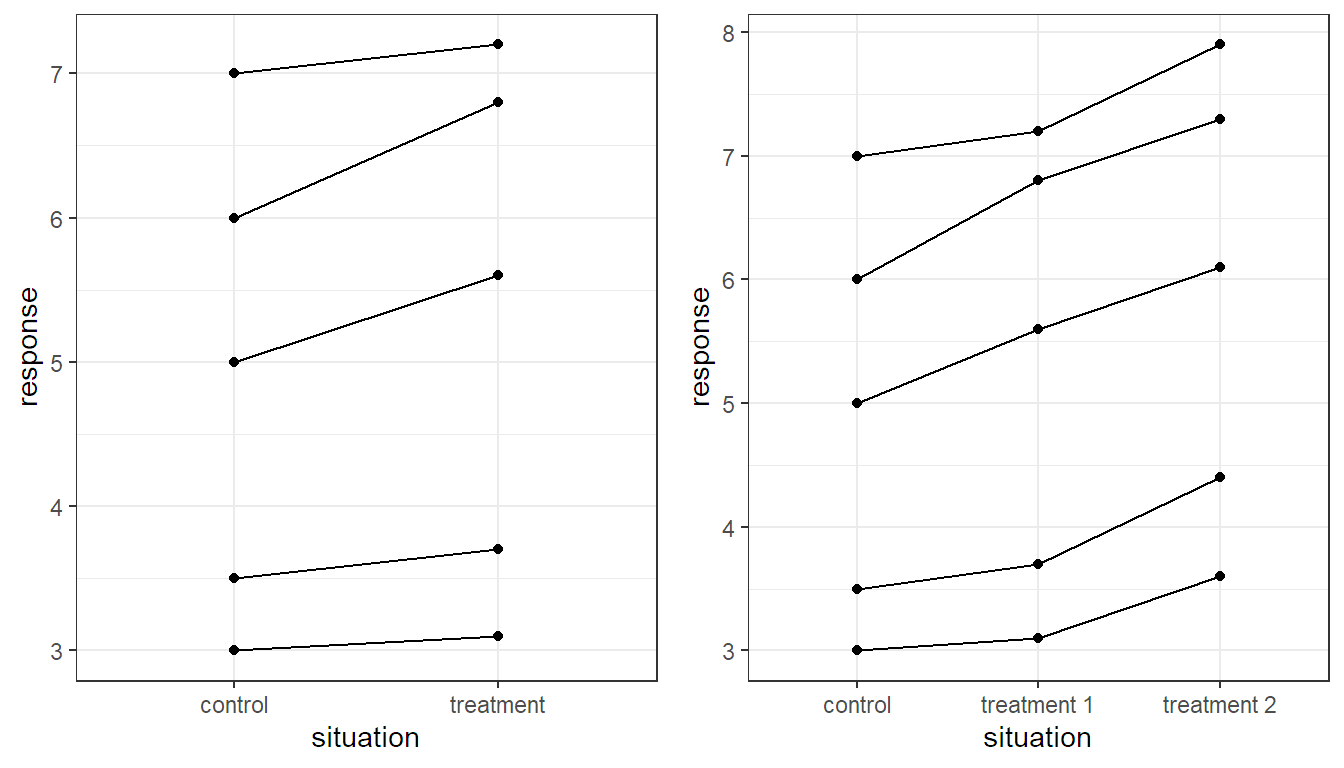
\includegraphics[width=\linewidth]{block-illustration.png}
\end{center}


\subsection{Randomized Complete Block Designs}

Assume that we can divide our experimental units into $r$ groups, also known as blocks, containing $g$ experimental units each. The \textbf{randomized complete block design} (RCBD) uses a restricted randomization scheme: Within every block, the $g$ treatments are randomized to the $g$ experimental units. The design is called complete because we observe the complete set of treatments within every block. Note that blocking is a special way to design an experiment, or a special "flavor" of randomization. It is not something that you use only when analyzing the data. \medskip

The experimental units should be as similar as possible within the same block, but can be very different between different blocks. This design allows us to fully remove the between-block variability from the response because it can be explained by the block factor. In that sense, blocking is a so-called variance reduction technique. The randomization step within each block makes sure that we are protected from unknown confounding variables. Typcial block factors are location, day, machine operator, subjects, etc. \medskip

In the most basic form, we assume that we do not have replicates within a block. This means that we only observe every treatment once in each block. The analysis of a randomized complete block design is straightforward. We treat the block factor as "just another" factor in our model. As we have no replicates within blocks, we can only fit a main effects model of the form:
$$Y_{ij} = \mu + \alpha_i + \beta_j + \epsilon_{ij}$$

According to this model, we implicitly assume that blocks only cause additive shifts. Or in other words, the treatment effects are always the same, no matter what block we consider. We would like the block factor to explain a lot of variation, hence if the mean square of the block factor is larger than the error mean square $MS_E$ we conclude that blocking was efficient


